\documentclass[a4paper]{exam}
\usepackage{amsmath,amssymb,amsthm}
\usepackage{listings}
\usepackage{xcolor} % Optional, for color
\usepackage{geometry}
\usepackage{graphicx}
\usepackage{hyperref}
\usepackage{float}
\usepackage{multirow}
\usepackage{array}
\usepackage{titling} % Required for the subtitle command
\usepackage{pythonhighlight}
\usepackage{tikz}
\usepackage{caption}
\usepackage[table]{xcolor}

\usetikzlibrary{arrows}

\definecolor{codegreen}{rgb}{0,0.6,0}
\definecolor{codegray}{rgb}{0.5,0.5,0.5}
\definecolor{codepurple}{rgb}{0.58,0,0.82}
\definecolor{backcolour}{rgb}{0.95,0.95,0.92}

\lstdefinestyle{mystyle}{
    backgroundcolor=\color{backcolour},   
    commentstyle=\color{codegreen},
    keywordstyle=\color{magenta},
    numberstyle=\tiny\color{codegray}, % Adjust font size and color
    stringstyle=\color{codepurple},
    basicstyle=\ttfamily\footnotesize,
    breakatwhitespace=false,         
    breaklines=true,                 
    captionpos=b,                    
    keepspaces=true,                 
    numbers=left, % Line numbers on the left
    numbersep=5pt,                  
    showspaces=false,                
    showstringspaces=false,
    showtabs=false,                  
    tabsize=2,
    firstnumber=1 % Start line numbers at 1
}


\lstset{style=mystyle}


\setlength{\droptitle}{-1.5in} % Adjust this value to decrease the spacing above the title

\title{EE-426 / CE-442:  Cryptography and Network Security\\
ASSIGNMENT NO.1}

\author{Syed Ahad Ali\\
sa07753\\
L1}


\date{\today}

\printanswers % This command enables the display of answers


\begin{document}

    \maketitle
    % \vspace{-3cm} % Adjust this value to decrease the spacing below the title

    \begin{center}
        \textbf{Fall 2024}\\
        \textbf{Habib University}\\
        \textbf{Dhanani School of Science \& Engineering}\\
        \textbf{TOTAL MARKS:100}\\
        \textbf{OBTAINED MARKS:}
    \end{center}

    % \vspace{1cm} % Adjust this value to decrease the spacing below the title

    \section*{Purpose}
    The purpose of this assignment is to help you apply the concepts of access control, security attacks, security services, and security mechanisms. In addition, concepts of modular arithmetic and concepts from number theory like extended Euclidean algorithm, linear Diophantine equation, residue matrices will be reinforced.

    \section*{Instructions}
    \begin{enumerate}
        \item This assignment should be done individually.
        \item All questions should be answered in black ink only.
        \item Scan your answer sheet and upload it on LMS before the due date.
    \end{enumerate}

    \section*{Grading Criteria}
    \begin{enumerate}
        \item Your assignments will be checked by the instructor.
        \item You may be asked to give a viva where you will be judged on whether you understood the questions yourself. If you are unable to correctly answer the question you have attempted, you may lose your marks.
        \item Zero will be given if the assignment is found to be plagiarized.
        \item Untidy work will result in a reduction of your points.
    \end{enumerate}

    \section*{Late Submission Penalty}
    \begin{itemize}
        \item 1-day late submission - 20\% deduction of the maximum allowable marks.
        \item 2-days late submission - 40\% deduction of the maximum allowable marks.
        \item No submission will be accepted after one week of the original deadline.
    \end{itemize}

    \pagebreak

    \section*{CLO Assessments}
    \begin{table}[h]
        \centering
        \begin{tabular}{|p{2cm}| p{10cm}| p{3cm}|} % Adjust the widths as needed
        \hline
        \multicolumn{2}{|c|}{Course Learning Outcomes} & \multicolumn{1}{c|}{CLO Assessed} \\ \hline
        CLO 1 & Apply the concepts from number theory and algebraic structures in understanding the design of cryptographic algorithms. & \makebox[3cm][c]{\raisebox{0.5\height}{\checkmark}} \\ \hline
        CLO 2 & Evaluate the suitability of message integrity, message authentication, and key management methods when applying in a given security scenario. & \\ \hline
        CLO 3 & Explain the setup, algorithms, and security issues in existing symmetric-key and asymmetric-key cryptosystems.         & \\ \hline
        CLO 4 & Apply cryptography-based network security technologies in the design of networked information systems. & \\ \hline
        \end{tabular}
    \end{table}


    \pagebreak
    \begin{questions}
        \question[5 $\times$ 2 = 10]
        For the DAC model discussed in Chapter 1, an alternative representation of the protection state is a directed graph. Each subject and each object in the protection state is represented by a node (a single node is used for an entity that is both subject and object). A directed line from a subject to an object indicates an access right, and the label on the link defines the access right.
        \begin{parts}
            \part
            Draw a directed graph that corresponds to the access matrix of the following Figure.
            \begin{table}[H]
                \centering
                \begin{tabular}{|c|c|c|c|c|}
                    \hline
                    & File 1 & File 2 & File 3 & File 4 \\ \hline
                    User A & Own, Read, Write & & Own, Read, Write & \\ \hline
                    User B & Read & Own, Read, Write & Write & Read \\ \hline
                    User C & Read, Write & Read & & Own, Read, Write \\ \hline
                \end{tabular}
            \end{table}
            \captionof{figure}{Access Matrix}
            
            \part
            Draw a directed graph that corresponds to the extended access matrix of the following Figure.
            \begin{table}[H]
                \begin{tabular}{|ccccccccccc|}
                    \hline
                    \multicolumn{11}{|c|}{OBJECTS}                                                                                                                                                                                                                                                                                                                                                                                                    \\ \hline
                    \multicolumn{2}{|c|}{\multirow{2}{*}{}}                                   & \multicolumn{3}{c|}{Subjects}                                                                                                              & \multicolumn{2}{c|}{Files}                                                                              & \multicolumn{2}{c|}{Processes}                            & \multicolumn{2}{c|}{Disk Drives}   \\ \cline{3-11} 
                    \multicolumn{2}{|c|}{}                                                    & \multicolumn{1}{c|}{S1}      & \multicolumn{1}{c|}{S2}      & \multicolumn{1}{c|}{S3}                                                      & \multicolumn{1}{c|}{F1}     & \multicolumn{1}{c|}{F2}                                                   & \multicolumn{1}{c|}{P1}     & \multicolumn{1}{c|}{P2}     & \multicolumn{1}{c|}{D1}    & D2    \\ \hline
                    \multicolumn{1}{|c|}{\multirow{3}{*}{SUBJECTS}} & \multicolumn{1}{c|}{S1} & \multicolumn{1}{c|}{Control} & \multicolumn{1}{c|}{Owner}   & \multicolumn{1}{c|}{\begin{tabular}[c]{@{}c@{}}Owner\\ Control\end{tabular}} & \multicolumn{1}{c|}{Read*}  & \multicolumn{1}{c|}{\begin{tabular}[c]{@{}c@{}}Read\\ Owner\end{tabular}} & \multicolumn{1}{c|}{Wakeup} & \multicolumn{1}{c|}{Wakeup} & \multicolumn{1}{c|}{Seek}  & Owner \\ \cline{2-11} 
                    \multicolumn{1}{|c|}{}                          & \multicolumn{1}{c|}{S2} & \multicolumn{1}{c|}{}        & \multicolumn{1}{c|}{Control} & \multicolumn{1}{c|}{}                                                        & \multicolumn{1}{c|}{Write*} & \multicolumn{1}{c|}{Execute}                                              & \multicolumn{1}{c|}{}       & \multicolumn{1}{c|}{}       & \multicolumn{1}{c|}{Owner} & Seek* \\ \cline{2-11} 
                    \multicolumn{1}{|c|}{}                          & \multicolumn{1}{c|}{S2} & \multicolumn{1}{c|}{}        & \multicolumn{1}{c|}{}        & \multicolumn{1}{c|}{Control}                                                 & \multicolumn{1}{c|}{}       & \multicolumn{1}{c|}{Write}                                                & \multicolumn{1}{c|}{Stop}   & \multicolumn{1}{c|}{}       & \multicolumn{1}{c|}{}      &       \\ \hline
                \end{tabular}
            \end{table}
            \captionof{figure}{Extended Access Control Matrix}
        \end{parts}
        \begin{solution}
            \begin{parts}
                \part
                \centering
                \begin{tikzpicture}[->, >=stealth', node distance=2cm, every node/.style={circle, draw, minimum size=1cm}]
                    % Nodes
                    \node (userA) at (0, 4) {User A};
                    \node (userB) at (10, 2) {User B};
                    \node (userC) at (0, -4) {User C};
                    
                    \node (file1) at (5, 7.5) {File 1};
                    \node (file2) at (5, 2.5) {File 2};
                    \node (file3) at (5, -2.5) {File 3};
                    \node (file4) at (5, -7.5) {File 4};
                
                    % Edges
                    \draw (userA) -- (file1) node[midway, above, draw=none] {Own, Read, Write};
                    \draw (userA) -- (file3) node[midway, above, draw=none] {Own, Read, Write};
                    
                    \draw (userB) -- (file1) node[midway, above, draw=none] {Read};
                    \draw (userB) -- (file2) node[midway, draw=none] {Own, Read, Write};
                    \draw (userB) -- (file3) node[midway, below, draw=none] {Write};
                    
                    \draw (userC) -- (file2) node[midway, below, draw=none] {Read};
                    \draw (userC) -- (file3) node[midway, below, draw=none] {Read};
                    \draw (userC) -- (file4) node[midway, below, draw=none] {Own, Read, Write};
                \end{tikzpicture}
                \captionof{figure}{Directed Graph for the Access Matrix}
                \part
                \begin{figure}[H]
                    \centering
                    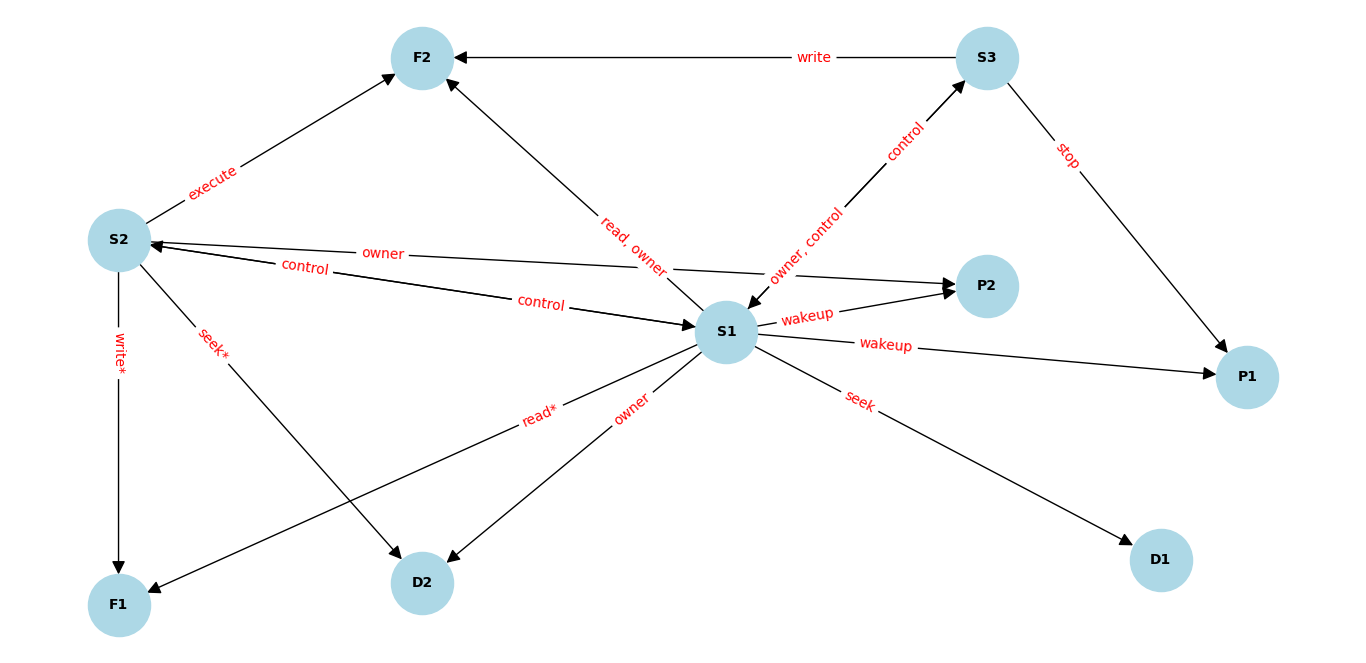
\includegraphics[width=0.7\textwidth]{./python/figure.png}
                    \caption{Directed Graph for the Extended Access Matrix (Note: There are directed edges from each subject node to themselves with the label of control)}
                \end{figure}
            \end{parts}
        \end{solution}

        \question[10]
        Using the Euclidean algorithm, find the greatest common divisor of the following pair of integers: 300 and 42.\\
        Also, based on the result, comment whether the pair is relatively-prime or not relatively-prime.
        \begin{solution}
            The algorithm is as follows:
            \begin{table}[H]
                \begin{center}
                    \begin{tabular}{|r|r|r|r|}
                        \hline
                        \multicolumn{1}{|c|}{\textbf{q}}                                      & \multicolumn{1}{c|}{\textbf{$r_1$}} & \multicolumn{1}{c|}{\textbf{$r_2$}} & \multicolumn{1}{c|}{\textbf{r}}                                      \\ \hline
                        7                                                                     & 300                                 & 42                                  & 6                                                                    \\ \hline
                        7                                                                     & 42                                  & 6                                   & 0                                                                    \\ \hline
                         & 6                                   & 0                                   &   \\ \hline
                    \end{tabular}
                \end{center}
            \end{table}
            The greatest common divisor of 300 and 42 is 6. Since the GCD is not 1, the pair is not relatively-prime.
        \end{solution}

        \pagebreak

        \question[10]
        Using the extended Euclidean algorithm, find the greatest common divisor of the following pair and the value of s and t: 400 and 60.

        \begin{solution}
            \begin{table}[H]
                \begin{center}
                    \begin{tabular}{cccccccccc}
                    \hline
                    \multicolumn{1}{|c|}{\textbf{q}}               & \multicolumn{1}{c|}{\textbf{$r_1$}} & \multicolumn{1}{c|}{\textbf{$r_2$}} & \multicolumn{1}{c|}{\textbf{r}}               & \multicolumn{1}{c|}{\textbf{$s_1$}} & \multicolumn{1}{c|}{\textbf{$s_2$}} & \multicolumn{1}{c|}{\textbf{s}}               & \multicolumn{1}{c|}{\textbf{$t_1$}} & \multicolumn{1}{c|}{\textbf{$t_2$}} & \multicolumn{1}{c|}{\textbf{t}}               \\ \hline
                    \multicolumn{1}{|c|}{6}                        & \multicolumn{1}{c|}{400}            & \multicolumn{1}{c|}{60}             & \multicolumn{1}{c|}{40}                       & \multicolumn{1}{c|}{1}              & \multicolumn{1}{c|}{0}              & \multicolumn{1}{c|}{1}                        & \multicolumn{1}{c|}{0}              & \multicolumn{1}{c|}{1}              & \multicolumn{1}{c|}{-6}                       \\ \hline
                    \multicolumn{1}{|c|}{1}                        & \multicolumn{1}{c|}{60}             & \multicolumn{1}{c|}{40}             & \multicolumn{1}{c|}{20}                       & \multicolumn{1}{c|}{0}              & \multicolumn{1}{c|}{1}              & \multicolumn{1}{c|}{-1}                       & \multicolumn{1}{c|}{1}              & \multicolumn{1}{c|}{-6}             & \multicolumn{1}{c|}{7}                        \\ \hline
                    \multicolumn{1}{|c|}{2}                        & \multicolumn{1}{c|}{40}             & \multicolumn{1}{c|}{20}             & \multicolumn{1}{c|}{0}                        & \multicolumn{1}{c|}{1}              & \multicolumn{1}{c|}{-1}             & \multicolumn{1}{c|}{3}                        & \multicolumn{1}{c|}{-6}             & \multicolumn{1}{c|}{7}              & \multicolumn{1}{c|}{-20}                      \\ \hline
                    \multicolumn{1}{|c|}{}                         & \multicolumn{1}{c|}{20}             & \multicolumn{1}{c|}{0}              & \multicolumn{1}{c|}{}                         & \multicolumn{1}{c|}{-1}             & \multicolumn{1}{c|}{3}              & \multicolumn{1}{c|}{}                         & \multicolumn{1}{c|}{7}              & \multicolumn{1}{c|}{-20}            & \multicolumn{1}{c|}{}                         \\ \hline
                    \multicolumn{1}{l}{}                           & \multicolumn{1}{l}{}                & \multicolumn{1}{l}{}                & \multicolumn{1}{l}{}                          & \multicolumn{1}{l}{}                & \multicolumn{1}{l}{}                & \multicolumn{1}{l}{}                          & \multicolumn{1}{l}{}                & \multicolumn{1}{l}{}                & \multicolumn{1}{l}{}                          
                    \end{tabular}
                \end{center}
            \end{table}
            The GCD of the pair 600 and 400 is 20. Value of s is -1 and t is 7.
        \end{solution}

        \question[2 $\times$ 5 = 10]
        Find the results of the following operations:
        \begin{parts}
            \part 22 mod 7 
            \part 140 mod 10 
            \part -78 mod 13 
            \part 0 mod 15 
            \part 144 mod 26 
        \end{parts}
        \begin{solution}
            \begin{parts}
                \part 22 $\equiv$ 1 (mod 7)
                \part 140 $\equiv$ 0 (mod 10)
                \part -78 $\equiv$ 0 (mod 13)
                \part 0 $\equiv$ 0 (mod 15)
                \part 144 $\equiv$ 14 (mod 26)
            \end{parts}
        \end{solution}

        \pagebreak

        \question[5]
        Perform the following operations using reduction first. 
        \begin{parts}
            \part (4223 + 17372) mod 10
            \part (424 $\times$ 32) mod 10
        \end{parts}

        \begin{solution}
            \begin{parts}
                \part
                \[
                    (4223 + 17372) \text{ mod } 10
                \]
                \[
                    (3 + 2) \text{ mod } 10
                \]
                \[
                    5 \text{ mod } 10 = 5
                \]
                \part
                \[
                    (424 \times 32) \text{ mod } 10
                \]
                \[
                    (4 \times 2) \text{ mod } 10
                \]
                \[
                    8 \text{ mod } 10 = 8
                \]
            \end{parts}
        \end{solution}

        \question[5]
        Let us assign numeric values to the uppercase alphabet (A = 0, B = 1, \ldots, Z = 25). We can now do modular arithmetic on the system using modulo 26.
        \begin{parts}
            \part What is (M + N) mod 26 in this system?
            \part What is (B + 6) mod 26 in this system? 
            \part What is (Z - 5) mod 26 in this system? 
            \part What is (A - 10) mod 26 in this system? 
            \part What is (D $\times$ 3) mod 26 in this system?
        \end{parts}

        \begin{solution}
            \begin{parts}
                \part
                \[
                    (M + N) \text{ mod } 26
                \]
                \[
                    (12 + 13) \text{ mod } 26
                \]
                \[
                    25 \text{ mod } 26 = 25
                \]
                \part
                \[
                    (B + 6) \text{ mod } 26
                \]
                \[
                    (1 + 6) \text{ mod } 26
                \]
                \[
                    7 \text{ mod } 26 = 7
                \]
                \part
                \[
                    (Z - 5) \text{ mod } 26
                \]
                \[
                    (25 - 5) \text{ mod } 26
                \]
                \[
                    20 \text{ mod } 26 = 20
                \]
                \part
                \[
                    (A - 10) \text{ mod } 26
                \]
                \[
                    (0 - 10) \text{ mod } 26
                \]
                \[
                    16 \text{ mod } 26 = 16
                \]
                \part
                \[
                    (D \times 3) \text{ mod } 26
                \]
                \[
                    (3 \times 3) \text{ mod } 26
                \]
                \[
                    9 \text{ mod } 26 = 9
                \]
            \end{parts}
        \end{solution}

        \question[5]
        Suppose we are given a set of residues with modulus 26 ($\text{Z}_{26}$): 
        \begin{parts}
            \part List all additive inverse pairs in modulus 26.
            \part List all multiplicative inverse pairs in modulus 26.
        \end{parts}

        \begin{solution}
            \begin{parts}
                \part
                \begin{itemize}
                    \item (0, 0)
                    \item (1, 25)
                    \item (2, 24)
                    \item (3, 23)
                    \item (4, 22)
                    \item (5, 21)
                    \item (6, 20)
                    \item (7, 19)
                    \item (8, 18)
                    \item (9, 17)
                    \item (10, 16)
                    \item (11, 15)
                    \item (12, 14)
                    \item (13, 13)
                \end{itemize}
                \part
                \begin{itemize}
                    \item (3, 9)
                    \item (5, 21)
                    \item (7, 15)
                    \item (11, 19)
                    \item (17, 23)
                    \item (25, 25)
                \end{itemize}
            \end{parts}
        \end{solution}

        \question[5]
        Find the multiplicative inverse of the following integer in ($\text{Z}_{180}$) using the extended Euclidean algorithm: 11.

        \begin{solution}
            \begin{table}[H]
                \begin{center}
                    \begin{tabular}{|r|r|r|r|r|r|r|}
                    \hline
                    \multicolumn{1}{|c|}{\textbf{q}}               & \multicolumn{1}{c|}{\textbf{$r_1$}} & \multicolumn{1}{c|}{\textbf{$r_2$}} & \multicolumn{1}{c|}{\textbf{r}}               & \multicolumn{1}{l|}{\textbf{$t_1$}} & \multicolumn{1}{l|}{\textbf{$t_2$}} & \multicolumn{1}{l|}{\textbf{t}}               \\ \hline
                    16                                             & 180                                 & 11                                  & 4                                             & 0                                   & 1                                   & -16                                           \\ \hline
                    2                                              & 11                                  & 4                                   & 3                                             & 1                                   & -16                                 & 33                                            \\ \hline
                    1                                              & 4                                   & 3                                   & 1                                             & -16                                 & 33                                  & -49                                           \\ \hline
                    3                                              & 3                                   & 1                                   & 0                                             & 33                                  & -49                                 & 180                                           \\ \hline
                    \multicolumn{1}{|l|}{}                         & 1                                   & 0                                   & \multicolumn{1}{l|}{}                         & -49                                 & 180                                 & \multicolumn{1}{l|}{} \\ \hline
                    \end{tabular}
                \end{center}
            \end{table}
            The multiplicative inverse of 11 from the table is -49. Since the inverse is negative, the positive value is 131.
        \end{solution}

        \question[10]
        A post office sells only 39-cent and 15-cent stamps. Find the number of stamps a customer needs to buy to put \$2.70 postage on a package. Find a few solutions.

        \begin{solution}
            Let $x$ be the number of 39-cent stamps and $y$ be the number of 15-cent stamps. The linear diophantine equation is:
            \[
                39x + 15y = 270
            \]
            By calculating the values of d, s, and t using the extended Euclidean algorithm;
            \begin{table}[H]
                \begin{center}
                    \begin{tabular}{|c|c|c|c|c|c|c|c|c|c|}
                    \hline
                    \textbf{q}               & \textbf{$r_1$} & \textbf{$r_2$} & \textbf{r}               & \textbf{$s_1$} & \textbf{$s_2$} & \textbf{s}               & \textbf{$t_1$} & \textbf{$t_2$} & \textbf{t}                                      \\ \hline
                    2                        & 39             & 15             & 9                        & 1                & 0              & 1                        & 0              & 1              & -2                                              \\ \hline
                    1                        & 15             & 9              & 6                        & 0                & 1              & -1                       & 1              & -2             & 3                                               \\ \hline
                    1                        & 9              & 6              & 3                        & 1                & -1             & 2                        & -2             & 3              & -5                                              \\ \hline
                    2                        & 6              & 3              & 0                        & -1               & 2              & -5                       & 3              & -5             & 13                                              \\ \hline
                                             & 3              & 0              &                          & 2                & -5             &                          & -5             & 13             &                                                 \\ \hline
                    \end{tabular}
                \end{center}
            \end{table}
            d = 3, s = 2, and t = -5.\\
            Infinite solutions exist as 3|270.\\
            Considering the solutions only where x and y both are positive integers, the equations are:
            \[
                x = \frac{c \times s + k \times b}{d}
            \]
            \[
                y = \frac{c \times t - k \times a}{d}
            \]
            For k $\in$ [-36, -35] we will have positive values of x \& y given as;
            \begin{table}[H]
                \begin{center}
                    \begin{tabular}{|c|c|c|}
                    \hline
                    \textbf{k} & \textbf{x} & \textbf{y} \\ \hline
                    -36        & 0        & 18         \\ \hline
                    -35        & 5        & 5         \\ \hline
                    \end{tabular}
                \end{center}
            \end{table}
            So the customer needs to buy 5 39-cent stamps and 5 15-cent stamps or just 18 15-cent stamps to put \$2.70 postage on a package.
        \end{solution}

        \question[10]
        Find all solutions to the following linear equation: 3x + 4 $\equiv$ 6 (mod 13).

        \begin{solution}
            \[
                3x + 4 \equiv 6 \text{ (mod 13)}
            \]
            \[
                3x + 4 + 9 \equiv 6 + 9 \text{ (mod 13)}
            \]
            \[
                3x \equiv 2 \text{ (mod 13)}
            \]
            The equation is of the form $ax \equiv b \text{ (mod m)}$. As d = 1 and 1|2, the equation has one solution:
            \[
                x \equiv (3^{-1} \times 2) \text{ (mod 13)}
            \]
            Finding the multiplicative inverse of 3 (mod 13):
            \begin{table}[H]
                \begin{center}
                    \begin{tabular}{|c|c|c|c|c|c|c|}
                    \hline
                    \textbf{q}               & \textbf{$r_1$} & \textbf{$r_2$} & \textbf{r}               & \textbf{$t_1$} & \textbf{$t_2$} & \textbf{t}               \\ \hline
                    4                        & 13             & 3              & 1                        & 0              & 1              & -4                       \\ \hline
                    3                        & 3              & 1              & 0                        & 1              & -4             & 13                       \\ \hline
                    & 1                                       & 0              &                          & -4             & 13             &                          \\ \hline
                    \end{tabular}
                \end{center}
            \end{table}
            The multiplicative inverse of 3 in ($\text{Z}_{13}$) is -4 $\equiv$ 9.
            \[
                x \equiv 9 \times 2 \text{ (mod 13)}
            \]
            \[
                x \equiv 18 \text{ (mod 13)}
            \]
            \[
                x \equiv 5 \text{ (mod 13)}
            \]
            So the solution to the equation is x = 5.
        \end{solution}

        \question[10]
        Find the determinant and the multiplicative inverse of each residue matrix over ($\text{Z}_{26}$):\\
        \[A=
            \begin{bmatrix}
                1 & 5 \\
                3 & 4
            \end{bmatrix}
        \]
        \[B=
            \begin{bmatrix}
                17 & 17 & 5 \\
                21 & 18 & 21 \\
                2 & 2 & 19
            \end{bmatrix}
        \]
        \begin{solution}
            \begin{parts}
                \part
                The inverse of a matrix A is given by:
                \[A^{-1} = \frac{\text{Adj}(A)}{\det(A)} \pmod{26}\]
                Since the matrix is 2x2, the determinant is calculated as:
                \[
                    \det(A) = 4 - 15 \pmod{26}
                \]
                \[
                    \det(A) = -11 \pmod{26}
                \]
                \[
                    \det(A) = 15 \pmod{26}
                \]
                From Question 7, the multiplicative inverse of 15 in ($\text{Z}_{26}$) is 7.
                For the adjoint matrix:
                \[
                    \begin{bmatrix}
                        4 & -5 \\
                        -3 & 1
                    \end{bmatrix}
                \]
                We take the modulo 26 of the negative values:
                \[
                    \begin{bmatrix}
                        4 & 21 \\
                        23 & 1
                    \end{bmatrix}
                \]
                Now the inverse of the matrix A can also be written as the following:
                \[
                    A^{-1} = \text{Adj}(A)\det(A)^{-1} \pmod{26}
                \]
                Since the determinant is 15 and its inverse is 7, the inverse of the matrix A is:
                \[A^{-1} = 
                    \begin{bmatrix}
                        4 & 21 \\
                        23 & 1
                    \end{bmatrix} \times 7 \pmod{26}
                \]
                \[A^{-1} = 
                    \begin{bmatrix}
                        28 & 147 \\
                        161 & 7
                    \end{bmatrix} \pmod{26}
                \]
                \[A^{-1} = 
                    \begin{bmatrix}
                        2 & 17 \\
                        5 & 7
                    \end{bmatrix} \pmod{26}
                \]
                \part
                The determinant of the matrix B is calculated as:
                \[
                    B^{-1} = \text{Adj}(B)\det(B)^{-1} \pmod{26}
                \]
                \[
                    \det(B) = 17(18 \times 19 - 2 \times 21) - 17(21 \times 19 - 2 \times 21) + 5(21 \times 2 - 18 \times 2) \pmod{26}
                \]
                \[
                    \det(B) = -939 \pmod{26}
                \]
                \[
                    \det(B) = 23 \pmod{26}
                \]
                From Question 7, the multiplicative inverse of 23 in ($\text{Z}_{26}$) is 17, So $\det(B)^{-1} = 17$.
                For the adjoint matrix:
                \[\text{Adj}(B)=
                    \begin{bmatrix}
                        (18\times19-2\times21) & -(21\times19-21\times2) & (21\times2-18\times2)\\
                        -(17\times19-5\times2) & (17\times19-5\times2) & -(17\times2-17\times2)\\
                        (17\times21-5\times18) & -(17\times21 - 5\times21) & (17\times18 - 17\times21)
                    \end{bmatrix}^{\text{T}} \pmod{26}
                \]
                After simplifying the matrix:
                \[\text{Adj}(B)=
                    \begin{bmatrix}
                        300 & -357 & 6\\
                        -313 & 313 & 0\\
                        267 & -252 & -51
                    \end{bmatrix}^{\text{T}} \pmod{26}
                \]
                After taking the modulo 26 of the negative values:
                \[\text{Adj}(B)=
                    \begin{bmatrix}
                        14 & 7 & 6\\
                        25 & 1 & 0\\
                        7 & 8 & 1
                    \end{bmatrix}^{\text{T}} \pmod{26}
                \]
                After taking the transpose of the matrix:
                \[\text{Adj}(B)=
                    \begin{bmatrix}
                        14 & 25 & 7\\
                        7 & 1 & 8\\
                        6 & 0 & 1
                    \end{bmatrix} \pmod{26}
                \]
                The inverse of the matrix B is:
                \[B^{-1} = 
                    \begin{bmatrix}
                        14 & 25 & 7\\
                        7 & 1 & 8\\
                        6 & 0 & 1
                    \end{bmatrix} \times 17 \pmod{26}
                \]
                \[B^{-1} =
                    \begin{bmatrix}
                        238 & 425 & 119\\
                        119 & 17 & 136\\
                        102 & 0 & 17
                    \end{bmatrix} \pmod{26}
                \]
                \[B^{-1} =
                    \begin{bmatrix}
                        4 & 9 & 15\\
                        15 & 17 & 6\\
                        24 & 0 & 17
                    \end{bmatrix} \pmod{26}
                \]
            \end{parts}
        \end{solution}

        \question[10]
        Find all solutions to the following sets of linear equations:
        \begin{parts}
            \part
            \[
                3x + 2y \equiv 5 \pmod{7}
            \]
            \[
                4x + 6y \equiv 4 \pmod{7}
            \]
            \part
            \[
                3x + 4y + 6z \equiv 9 \pmod{10}
            \]
            \[
                x + y + 8z \equiv 7 \pmod{10}
            \]
            \[
                5x + 8y + 3z \equiv 0 \pmod{10}
            \]
        \end{parts}
        \begin{solution}
            \begin{parts}
                \part
                Given;
                \[
                    3x + 2y \equiv 5 \pmod{7}
                \]
                \[
                    4x + 6y \equiv 4 \pmod{7}
                \]
                We can rewrite the equations as;
                \[
                    \begin{bmatrix}
                        3 & 2\\
                        4 & 6
                    \end{bmatrix}\begin{bmatrix}
                        x\\y
                    \end{bmatrix} \equiv \begin{bmatrix}
                        5\\4
                    \end{bmatrix}
                \]
                Where the matrix $\text{A}_x$, $\text{A}_y$, and A are:
                \[
                    A_x = \begin{bmatrix}
                        5 & 2\\
                        4 & 6
                    \end{bmatrix}
                \]
                \[
                    A_y = \begin{bmatrix}
                        3 & 5\\
                        4 & 4
                    \end{bmatrix}
                \]
                \[
                    A = \begin{bmatrix}
                        3 & 2\\
                        4 & 6
                    \end{bmatrix}
                \]

                From Cramer's rule;
                \[
                    x = \frac{\det(A_x)}{\det(A)}
                \]
                \[
                    y = \frac{\det(A_y)}{\det(A)}
                \]
                Or;
                \[
                    x = \det(A_x) \times \det(A)^{-1}
                \]
                \[
                    y = \det(A_y) \times \det(A)^{-1}
                \]
                Calculating the determinants:
                \[
                    \det(A) = 18 - 8 \pmod{7}
                \]
                \[
                    \det(A) = 10 \equiv 3 \pmod{7}
                \]
                \[
                    \det(A_x) = 30 - 8 \pmod{7}
                \]
                \[
                    \det(A_x) = 22 \equiv 1 \pmod{7}
                \]
                \[
                    \det(A_y) = 12 - 20 \pmod{7}
                \]
                \[
                    \det(A_y) = -8 \equiv 6 \pmod{7}
                \]
                Calculating the value of $\det(A)^{-1}$ in ($\text{Z}_{7}$) using the extended Euclidean algorithm:
                \begin{table}[H]
                    \begin{center}
                        \begin{tabular}{|r|r|r|r|r|r|r|}
                            \hline
                            \multicolumn{1}{|c|}{\textbf{q}}               & \multicolumn{1}{c|}{\textbf{$r_1$}} & \multicolumn{1}{c|}{\textbf{$r_2$}} & \multicolumn{1}{c|}{\textbf{r}}               & \multicolumn{1}{c|}{\textbf{$t_1$}} & \multicolumn{1}{c|}{\textbf{$t_2$}} & \multicolumn{1}{c|}{\textbf{t}}               \\ \hline
                            2                                              & 7                                   & 3                                   & 1                                             & 0                                     & 1                                   & -2                                            \\ \hline
                            3                                              & 3                                   & 1                                   & 0                                             & 1                                     & -2                                  & 7                                             \\ \hline
                            \multicolumn{1}{|l|}{}                         & 1                                   & 0                                   & \multicolumn{1}{l|}{}                         & -2                                    & 7                                   & \multicolumn{1}{l|}{}                         \\ \hline
                        \end{tabular}
                    \end{center}
                \end{table}
                The multiplicative inverse of 3 in ($\text{Z}_{7}$) is -2 $\equiv$ 5.
                Calculating the values of x and y:
                \[
                    x = 1 \times 5 \pmod{7}
                \]
                \[
                    x = 5 \pmod{7}
                \]
                \[
                    y = 6 \times 5 \pmod{7}
                \]
                \[
                    y = 30 \pmod{7}
                \]
                \[
                    y = 2 \pmod{7}
                \]
                So the solutions to the equations are x = 5 and y = 2.
                \part
                Given;
                \[
                    3x + 4y + 6z \equiv 9 \pmod{10}
                \]
                \[
                    x + y + 8z \equiv 7 \pmod{10}
                \]
                \[
                    5x + 8y + 3z \equiv 0 \pmod{10}
                \]
                We can rewrite the equations as;
                \[
                    \begin{bmatrix}
                        3 & 4 & 6\\
                        1 & 1 & 8\\
                        5 & 8 & 3
                    \end{bmatrix}\begin{bmatrix}
                        x\\y\\z
                    \end{bmatrix} \equiv \begin{bmatrix}
                        9\\7\\0
                    \end{bmatrix}
                \]
                Where the matrix $\text{A}_x$, $\text{A}_y$, $\text{A}_z$, and A are:
                \[
                    A_x = \begin{bmatrix}
                        9 & 4 & 6\\
                        7 & 1 & 8\\
                        0 & 8 & 3
                    \end{bmatrix}
                \]
                \[
                    A_y = \begin{bmatrix}
                        3 & 9 & 6\\
                        1 & 7 & 8\\
                        5 & 0 & 3
                    \end{bmatrix}
                \]
                \[
                    A_z = \begin{bmatrix}
                        3 & 4 & 9\\
                        1 & 1 & 7\\
                        5 & 8 & 0
                    \end{bmatrix}
                \]
                \[
                    A = \begin{bmatrix}
                        3 & 4 & 6\\
                        1 & 1 & 8\\
                        5 & 8 & 3
                    \end{bmatrix}
                \]
                From Cramer's rule;
                \[
                    x = \frac{\det(A_x)}{\det(A)}
                \]
                \[
                    y = \frac{\det(A_y)}{\det(A)}
                \]
                \[
                    z = \frac{\det(A_z)}{\det(A)}
                \]
                Or;
                \[
                    x = \det(A_x) \times \det(A)^{-1}
                \]
                \[
                    y = \det(A_y) \times \det(A)^{-1}
                \]
                \[
                    z = \det(A_z) \times \det(A)^{-1}
                \]
                Calculating the determinants:
                \[
                    \det(A) = 3 \begin{vmatrix} 1 & 8 \\ 8 & 3 \end{vmatrix} - 4 \begin{vmatrix} 1 & 8 \\ 5 & 3 \end{vmatrix} + 6 \begin{vmatrix} 1 & 1 \\ 5 & 8 \end{vmatrix}
                \]
                \[    = 3 (1 \cdot 3 - 8 \cdot 8) - 4 (1 \cdot 3 - 5 \cdot 8) + 6 (1 \cdot 8 - 1 \cdot 5)\]
                \[    = 3 (3 - 64) - 4 (3 - 40) + 6 (8 - 5)\]
                \[    = 3 \cdot (-61) - 4 \cdot (-37) + 6 \cdot 3\]
                \[    = -183 + 148 + 18\]
                \[    = -17 \pmod{10}\]
                \[    = 3 \pmod{10}\]

                \[    \det(A_x) = 9 \begin{vmatrix} 1 & 8 \\ 8 & 3 \end{vmatrix} - 4 \begin{vmatrix} 7 & 8 \\ 0 & 3 \end{vmatrix} + 6 \begin{vmatrix} 7 & 1 \\ 0 & 8 \end{vmatrix}\]
                \[    = 9 (1 \cdot 3 - 8 \cdot 8) - 4 (7 \cdot 3 - 8 \cdot 0) + 6 (7 \cdot 8 - 1 \cdot 0)\]
                \[    = 9 (3 - 64) - 4 (21) + 6 (56)\]
                \[    = 9 \cdot (-61) - 4 \cdot 21 + 6 \cdot 56\]
                \[    = -549 - 84 + 336\]
                \[    = -297 \pmod{10}\]
                \[    = 3 \pmod{10}\]

                \[    \det(A_y) = 3 \begin{vmatrix} 7 & 8 \\ 0 & 3 \end{vmatrix} - 9 \begin{vmatrix} 1 & 8 \\ 5 & 3 \end{vmatrix} + 6 \begin{vmatrix} 1 & 7 \\ 5 & 0 \end{vmatrix}\]
                \[    = 3 (7 \cdot 3 - 8 \cdot 0) - 9 (1 \cdot 3 - 5 \cdot 8) + 6 (1 \cdot 0 - 7 \cdot 5)\]
                \[    = 3 (21) - 9 (3 - 40) + 6 (0 - 35)\]
                \[    = 3 \cdot 21 - 9 \cdot (-37) + 6 \cdot (-35)\]
                \[    = 63 + 333 - 210\]
                \[    = 186 \pmod{10}\]
                \[    = 6 \pmod{10}\]

                \[    \det(A_z) = 3 \begin{vmatrix} 1 & 7 \\ 8 & 0 \end{vmatrix} - 4 \begin{vmatrix} 1 & 7 \\ 5 & 0 \end{vmatrix} + 9 \begin{vmatrix} 1 & 1 \\ 5 & 8 \end{vmatrix}\]
                \[    = 3 (1 \cdot 0 - 7 \cdot 8) - 4 (1 \cdot 0 - 7 \cdot 5) + 9 (1 \cdot 8 - 1 \cdot 5)\]
                \[    = 3 (0 - 56) - 4 (0 - 35) + 9 (8 - 5)\]
                \[    = 3 \cdot (-56) - 4 \cdot 35 + 9 \cdot 3\]
                \[    = -168 - 140 + 27\]
                \[    = -281 \pmod{10}\]
                \[    = -1 \pmod{10}\]
                \[    = 9 \pmod{10}\]

                Calculating the value of $\det(A)^{-1}$ in ($\text{Z}_{10}$) using the extended Euclidean algorithm:
                \begin{table}[H]
                    \begin{center}
                        \begin{tabular}{|c|c|c|c|c|c|c|}
                        \hline
                        \textbf{q}               & \textbf{$r_1$} & \textbf{$r_2$} & \textbf{r}               & \textbf{$t_1$} & \textbf{$t_2$} & \textbf{t}               \\ \hline
                        3                        & 10             & 3              & 1                        & 0              & 1              & -3                       \\ \hline
                        3                        & 3              & 1              & 0                        & 1              & -3             & 10                       \\ \hline
                                                 & 1              & 0              &                          & -3             & 10             &                          \\ \hline
                        \end{tabular}
                    \end{center}
                \end{table}
                The multiplicative inverse of 3 in ($\text{Z}_{10}$) is -3 $\equiv$ 7.
                Calculating the values of x, y, and z:
                \[
                    x = 3 \times 7 \pmod{10}
                \]
                \[
                    x = 21 \pmod{10}
                \]
                \[
                    x = 1 \pmod{10}
                \]
                \[
                    y = 6 \times 7 \pmod{10}
                \]
                \[
                    y = 42 \pmod{10}
                \]
                \[
                    y = 2 \pmod{10}
                \]
                \[
                    z = 9 \times 7 \pmod{10}
                \]
                \[
                    z = 63 \pmod{10}
                \]
                \[
                    z = 3 \pmod{10}
                \]
                So the solutions to the equations are x = 1, y = 2, and z = 3.
            \end{parts}
        \end{solution}
    \end{questions}
\end{document}